\section{Conformational Fluctuations of the ds and ss Rotaxanes}

Having gained insight into the entropic interactions between the DNA and the
nanopore in the mixed rotaxanes, now the stable intermediate states of the nanopiston's
operation cycle are
studied. Both the rotaxane-ss and -ds are composed of stiff dsDNA and flexible ssDNA
parts, which characterise their conformational fluctuations by the entropic interactions.
The two rotaxanes types are simulated in a nanopore, using the predefined coarse-grained
model, in absence of an external bias, i.e.  $0\ mV$. The results are presented in Figure
\ref{fig:conform}

Analysing the conformational fluctuations of the rotaxane-ds, we observe that the ssDNA
toehold remains predominantly outside of the pore. This effect can be explained by taking
into account the entropic cost of capturing the flexible strand of ssDNA into the
constriction of the pore. Since the geometry of the rotaxane prohibits the toehold from
reaching the cis-side of the pore, the toehold can only freely fluctuate on the
trans-side of the pore. Throughout the simulation this entropic force keeps the toehold
in the trans-reservoir and thereby placing the cis-protein stopper close to the entrance
of the pore. This entropic interaction plays an important role in the operation of the
nanopiston. Even when an external voltage difference induces an upward electrophoretic
force on the rotaxane, the competing entropic force keeps the toehold outside of the
constriction and thereby exposing it for hybridisation with a fuel strand. This also
explains the halting of the piston cycle at high voltages. In this case the entropic
force is overcome by the induced electrophoretic force, sequestering the toehold inside
of the pore inhibiting the binding of fuel strands.

In the same figure the results for the rotaxane-ss are presented. An upwards entropic
force is observed in the positional histograms, arising from the high flexibility of the
long ssDNA strand. This force originates from the increase in configurational microstates
available to the rotaxane-ss, when the ssDNA strand is allowed to freely fluctuate in the
cis-reservoir. The flexibility of the ssDNA strand overcomes the entropic penalty of
confining the dsDNA into the constriction of the pore. Capturing the interface between
the ssDNA and dsDNA parts of the rotaxane-ss inside of the pore promotes the
operation cycle. In this case a longer ssDNA strand is exposed to the cis-reservoir,
better facilitating the hybridisation with cargo strands. This can be seen in the
positional histogram of the cis-protein stopper, where the large fluctuations of the
ssDNA strand allow it to venture far away from the nanopore.

These results explain the functional importance of the entropic interactions in the
nanopiston's operating cycle. Comparing our findings with the simulation results by
Bayoumi et al.,
we see that both models are in reasonable accordance. However, in our simulations the
interface of the rotaxane-ss is observed entering inside the pore's constriction, while
in the bead-and-spring model this behaviour is not observed. This difference can be
attributed to the more accurate simulating of ssDNA by OxDNA, mainly arising from the
more precise parametrisation of the model and the ability for consecutive bases to
unstack.

\begin{figure}[ht!]
\begin{center}
  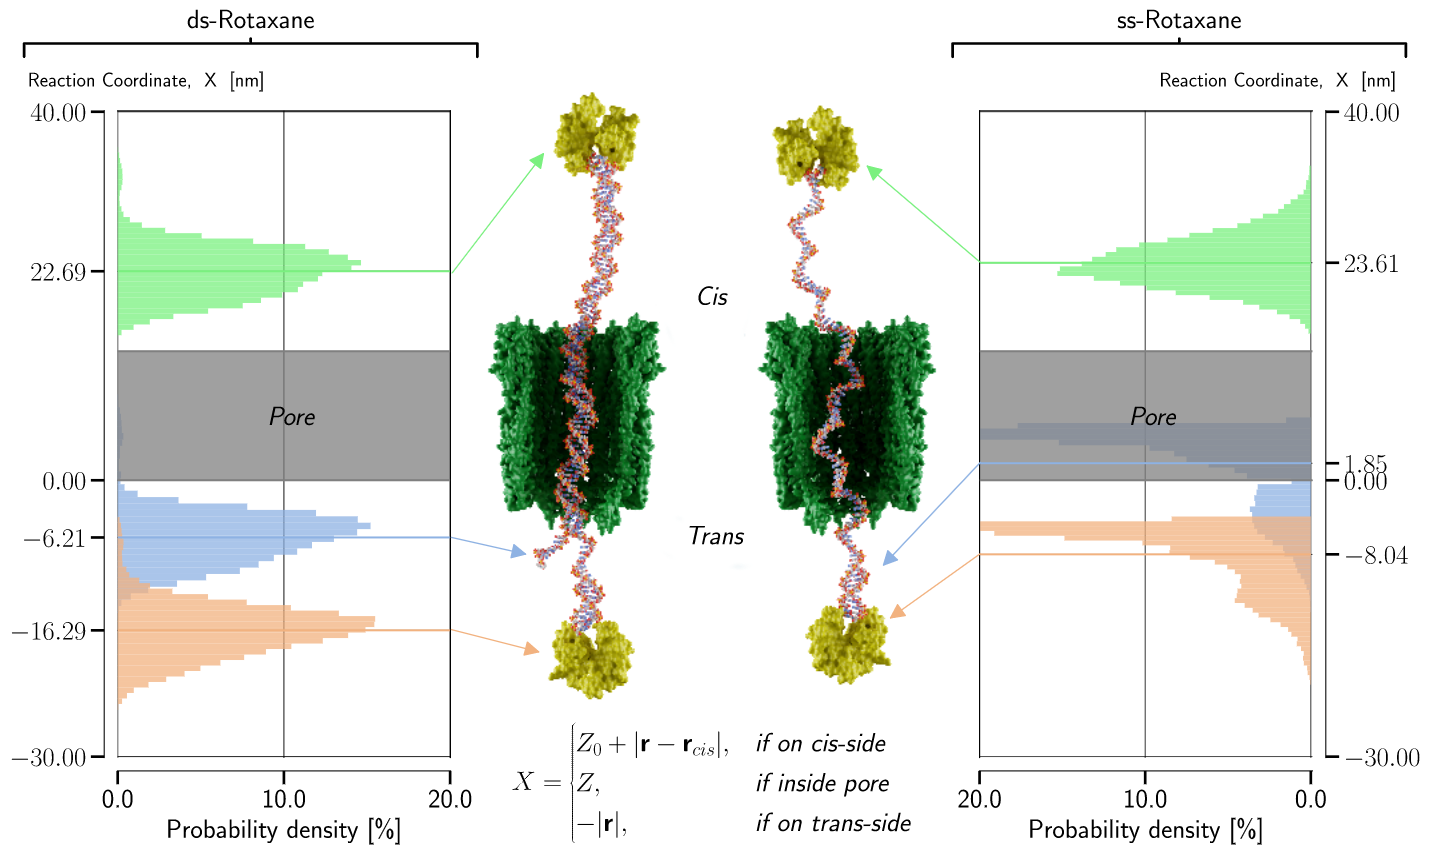
\includegraphics[width=1\textwidth]{Figures/image.png}
%   \caption[]{\linespread{0.5}{\small Entropic piston cycles. (a) Current traces showing
% the nanopiston cycling between the rotaxane-ds (purple) and rotaxane-ss (green)
% conformations, under a constant bias of−20 mV (top) and −20 mV (bottom) bias. The
% transition is induced through hybridization with the fuel and cargo in the trans and cis
% chambers. The gray horizontal lines indicate the average currents in rotaxane-ds and
% rotaxane-ss, labeled with Ld and Ls, respectively. Note that, the analysis of the
% rotaxane-ss current at −20 mV reveals two sublevels, Ls1 and Ls2 (see Section S6). (b)
% Schematic representation of the proposed states involved in a full cycle. The top and
% bottom states are the likely short-lived intermediate states (indicated byan asterisk).
% The electrical recordings were carried out at +20mVin 2MNaCl, 15mMTris-HCl, pH 7.5 at 22
% °C. Data were recorded by applying a 2 kHz low-pass Bessel filter, using a 100 μs (10
% kHz) sampling rate.
% 764}}
\end{center}
\label{fig:conform}
\end{figure}
